\documentclass[utf8x, 12pt]{G7-32} 
\sloppy

% Настройки стиля ГОСТ 7-32
% Для начала определяем, хотим мы или нет, чтобы рисунки и таблицы нумеровались в пределах раздела, или нам нужна сквозная нумерация.

%\EqInChapter % формулы будут нумероваться в пределах раздела
%\TableInChapter % таблицы будут нумероваться в пределах раздела
%\PicInChapter % рисунки будут нумероваться в пределах раздела

% Добавляем гипертекстовое оглавление в PDF
\usepackage[
bookmarks=true, colorlinks=true, unicode=true,
urlcolor=black,linkcolor=black, anchorcolor=black,
citecolor=black, menucolor=black, filecolor=black,
]{hyperref}

% Изменение начертания шрифта --- после чего выглядит таймсоподобно.
% apt-get install scalable-cyrfonts-tex

\IfFileExists{cyrtimes.sty}
    {
        \usepackage{cyrtimespatched}
    }
    {
        % А если Times нету, то будет CM...
    }

\usepackage{graphicx}   % Пакет для включения рисунков
\DeclareGraphicsExtensions{.jpg,.pdf,.png}
% С такими оно полями оно работает по-умолчанию:
% \RequirePackage[left=20mm,right=10mm,top=20mm,bottom=20mm,headsep=0pt]{geometry}
% Если вас тошнит от поля в 10мм --- увеличивайте до 20-ти, ну и про переплёт не забывайте:
\geometry{right=20mm}
\geometry{left=30mm}



% Произвольная нумерация списков.
\usepackage{enumerate}

\setcounter{tocdepth}{3} %Подробность оглавления
%4 это chapter, section, subsection, subsubsection и paragraph
%3 это chapter, section, subsection и subsubsection
%2 это chapter, section, и subsection
%1 это chapter и section
%0 это chapter.



\begin{document}

\frontmatter 
\begin{center} 

\large САНКТ-ПЕТЕРБУРГСИЙ ГОСУДАРСТВЕННЫЙ ПОЛИТЕХНИЧЕСКИЙ УНИВЕРСИТЕТ

\large Кафедра Компьютерных Систем и Программных Технологий \\[4.5cm] 

\huge ОТЧЕТ \\[0.6cm] % название работы, затем отступ 0,6см
\large по лабораторной работе №1\\
\large Тема: <<Основные виды анализа аналоговых электронных устройств в среде проектирования Cadence Allegro>>\\
\large Дисциплина: <<Автоматическое проектирование аналоговых цифровых устройств>>\\[2.7cm]

\end{center} 

\begin{flushright}
Выполнили: студенты гр. 53501/2 \\
Пономарев М.A \\
Федоров Е.М \\[1.2cm]

Преподаватель \\
Балтруков Н.Н
\end{flushright}


\vfill 

\begin{center} 
\large Санкт-Петербург \\
2015
\end{center} 

\thispagestyle{empty}

\thispagestyle{empty}
\setcounter{page}{0}
\tableofcontents
\clearpage
\mainmatter



\chapter{Цель работы}

Целью данной работы является изучение возможностей систем Cadence OrCAD (Allegro) по проектированию схемотехнических реализаций аналоговых электронных устройств, а также практики проведения основных видов анализа в симуляторе Cadence PSpice A/D.


\chapter{Программа работы}

\section{Подготовка}

В ходе подготовки к выполнению лабораторной работы был создан <<Analog or Mixed A/D>> проект <<lab2>> с подключением определенных библиотек для создания последующих принципиальных схем. 


\section{Анализ во временной области}
 
\subsection{Обычный анализ}
 
При использования редактора форм была создана принципиальная схема инвертирующего усилителя с коэффициентом усиления $k = 2$. 


\begin{figure}[h]
	\begin{center}
		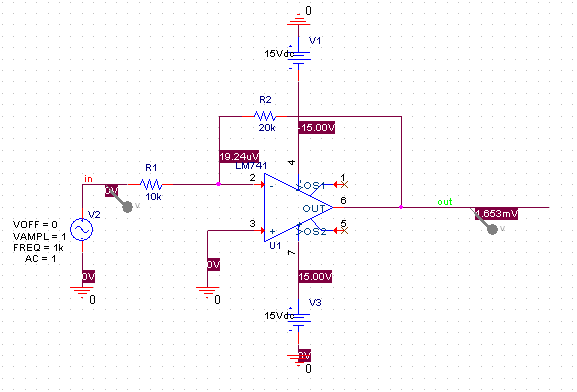
\includegraphics[width=12cm]{img/shema_1}
	\end{center}
	\vspace{-5mm}\caption{Схема инвертирующего усилителя для анализа во временной области}
\end{figure}	

Создадим файл симуляции <<mySim1>> со следующими настройками:

\begin{itemize}
	\item Analysis
	\begin{itemize}	
		\item Time Domain
		\begin{itemize}	
			\item Run to time = 10 ms
			\item Maximum step size = 500 ns
		\end{itemize}
	\end{itemize}
\end{itemize}

\newpage

\begin{figure}[h]
	\begin{center}
		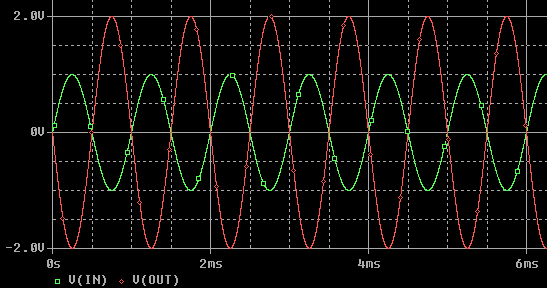
\includegraphics[width=7.5cm, height=4.5cm]{img/waveform_1_0}
		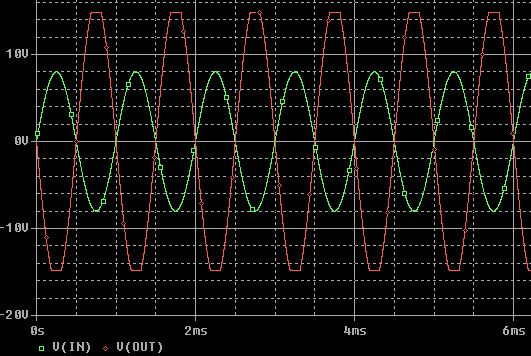
\includegraphics[width=7.5cm, height=4.5cm]{img/waveform_1_1}
	\end{center}
	\vspace{-5mm}\caption{Временные диаграммы переходных процессов при напряжении от источника входного сигнала равного 2V и 8V соответственно}
\end{figure}	

\subsection{Параметрический анализ}
Параметрический анализ во временной области позволяет получить семейство временных диаграмм на одном или нескольких графиках при варьировании определённого параметра схемы. (в нашем случае коэффициента усиления)

Для данного анализа модифицируем схему с добавлением элемента PARAM из библиотеки SPECIAL. После задания настроек этого элемента и изменения схемы, получаем следующую принципиальную схему.

\begin{figure}[h]
	\begin{center}
		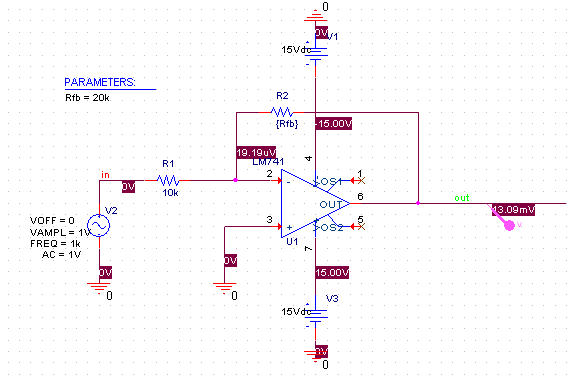
\includegraphics[width=12cm]{img/shema_2}
	\end{center}
	\vspace{-5mm}\caption{Параметризованная схема инвертирующего масштабного усилителя}
\end{figure}	

Создадим файл симуляции <<mySim2>> со следующими настройками:

\begin{itemize}
	\item Analysis
	\begin{itemize}	
		\item Time Domain (General Settings)
		\begin{itemize}	
			\item Run to time = 10 ms
			\item Maximum step size = 500 ns
		\end{itemize}
		\item Time Domain (Parametric Sweep)
		\begin{itemize}	
			\item Sweep variable --- <<Global parameter>>
			\item Parameter name --- <<Rfb>>
			\item Sweep type (Value list) = <<10k 20k 40k 80k 160k>>
		\end{itemize}
	\end{itemize}
\end{itemize}



\begin{figure}[h]
	\begin{center}
		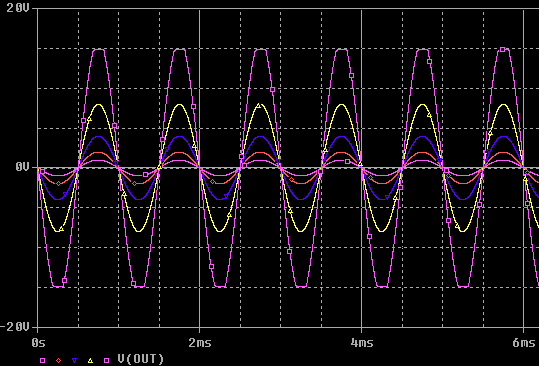
\includegraphics[width=7cm]{img/wavefrom_1_2}
	\end{center}
	\vspace{-5mm}\caption{Моделирование параметризованной схемы инвертирующего масштабного усилителя в зависимости от величины сопротивления в цепи обратно связи}
\end{figure}	

\newpage
\section{Анализ на постоянном токе}

\subsection{При заданных постоянных воздействиях}

Анализ на постоянном токе предполагает получение конкретного значения напряжения при заданных постоянных воздействиях.

Для анализа модифицируем схему, заменив источник напряжения VSIN на VDC. В результате получаем следующую принципиальную схему:

\begin{figure}[h]
	\begin{center}
		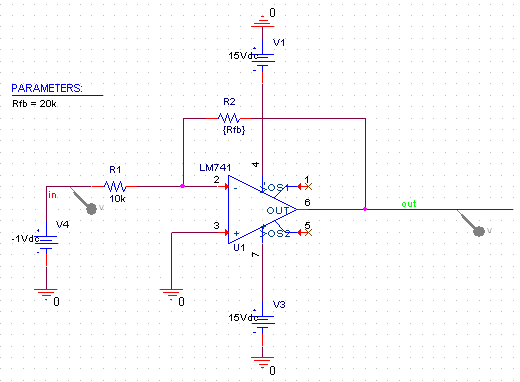
\includegraphics[width=12cm]{img/shema_3}
	\end{center}
	\vspace{-5mm}\caption{Схема инвертирующего масштабного усилителя для анализа на постоянном токе}
\end{figure}	

Создадим файл симуляции <<mySim3>> со следующими настройками:

	\begin{itemize}	
		\item Analysis type --- <<DC Sweep>>
		\begin{itemize}	
			\item Sweep variable
			\begin{itemize}	
				\item Voltage source --- <<V4>>
			\end{itemize}
			\item Sweep type -- <<Linear>>
			\begin{itemize}	
				\item Start value --- <<-16V>>
				\item End value --- <<16V>>
 				\item Increment --- <<0.1V>>
			\end{itemize}
		\end{itemize}
	\end{itemize}

\newpage

\begin{figure}[h]
	\begin{center}
		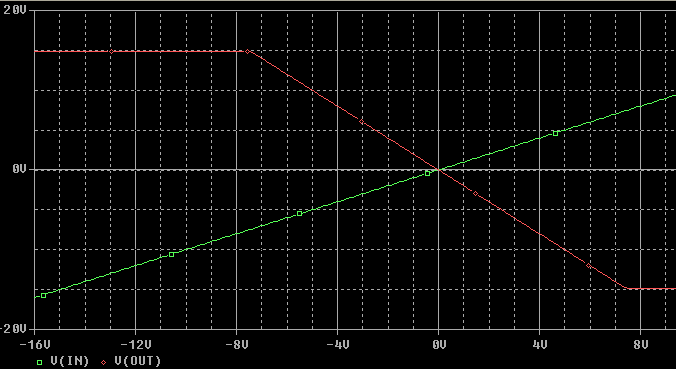
\includegraphics[width=12cm]{img/waveform_2_0}
	\end{center}
	\vspace{-5mm}\caption{Временная диаграмма анализа на постоянном токе}
\end{figure}	


\subsection{При вариации параметра схемы}

Создадим файл симуляции <<mySim4>>, скопируем настройки с <<mySim3>> и добавим следующие:

	\begin{itemize}	
		\item Analysis type --- <<DC Sweep>> --- <<Parametric Sweep>>
		\begin{itemize}	
			\item Sweep variable
			\begin{itemize}	
				\item Global parameter --- <<Rfb>>
			\end{itemize}
			\item Sweep type -- <<Value list>>
			\begin{itemize}	
				\item Value list --- <<10k 20k 40k>>
			\end{itemize}
		\end{itemize}
	\end{itemize}

\begin{figure}[h]
	\begin{center}
		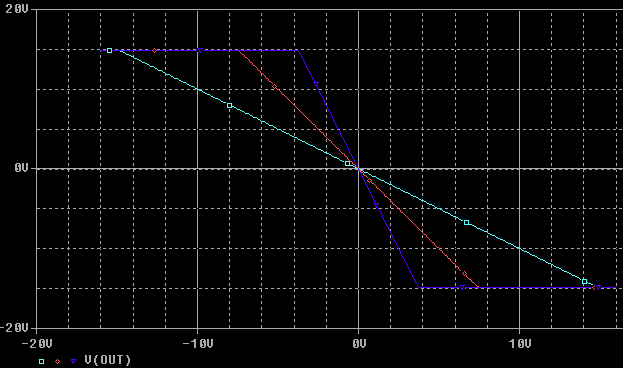
\includegraphics[width=12cm]{img/waveform_2_1}
	\end{center}
	\vspace{-5mm}\caption{Передаточные характеристики усилителя}
\end{figure}	

\newpage


\section{Анализ на переменном токе}

Для анализа на переменном токе рассматриваемого усилительного каскада, изменим схему эксперимента, вернув источник входного синусоидального напряжения и добавив на вход разделительный конденсатор, тем самым превратив схему в усилитель переменного напряжения:

\begin{figure}[h]
	\begin{center}
		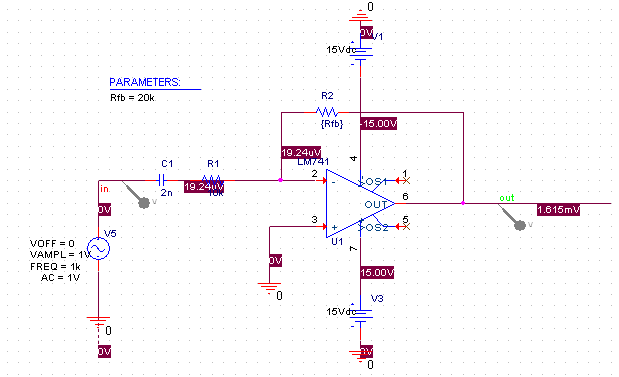
\includegraphics[width=12cm]{img/shema_4}
	\end{center}
	\vspace{-5mm}\caption{Схема усилителя переменного тока}
\end{figure}	


Создадим файл симуляции <<mySim5>> со следующими настройками:

	\begin{itemize}	
		\item Analysis type --- <<AC Sweep>>
		\begin{itemize}	
			\item Geberal Settings
			\begin{itemize}	
				\item Sweep type --- <<Logarimic (decade)>>
				\item Start frequency = 100
				\item End frequency = 100000000
				
			\end{itemize}
		\end{itemize}
	\end{itemize}

\begin{figure}[h]
	\begin{center}
		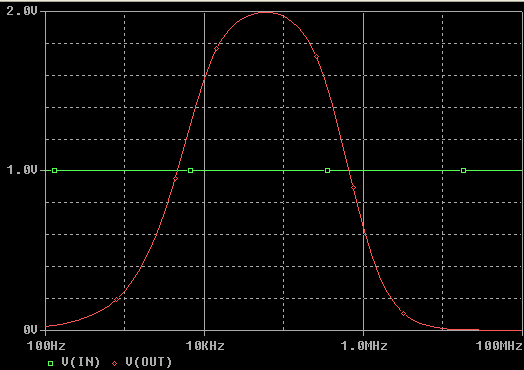
\includegraphics[width=7cm, height=5cm]{img/waveform_3_0}
		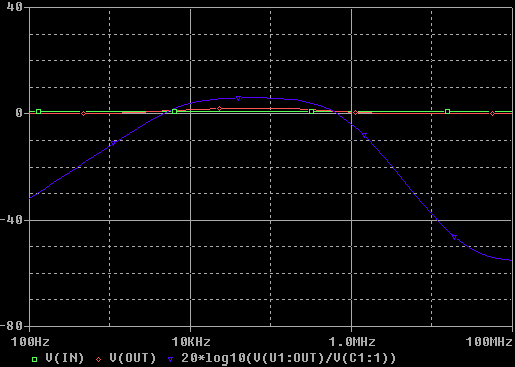
\includegraphics[width=7cm, height=5cm]{img/waveform_3_1}
	\end{center}
	\vspace{-5mm}\caption{Временная диаграмма анализа на переменном токе и ЛАЧХ}
\end{figure}	





\chapter{Выводы}
В ходе выполнения первой лабораторной работы были изучены основные возможности проектирования электронных устройств в среде OrCad. Кроме этого были изучены основные виды анализа принципиальных схем на постоянном и переменном токах.


\end{document}
